\documentclass[conference]{IEEEtran} 
\IEEEoverridecommandlockouts
\usepackage{amsmath,amssymb}
\usepackage{siunitx}
\usepackage{graphicx}
\usepackage{cite}
\usepackage[hidelinks]{hyperref} % ← これを追加(\url を定義)
\sisetup{detect-all=true}

\title{Low-Cost Integration of 1.8-V FeFET on 0.18-\(\mu\)m CMOS:\\
+1 Mask and a Single ALD Tool, with Reliability Assessment}

\author{%
Shinichi Samizo\\
\emph{Independent Semiconductor Researcher}\\
Former Engineer at Seiko Epson Corporation\\
Email: \texttt{shin3t72@gmail.com}\\
GitHub: \url{https://github.com/Samizo-AITL}
}
 
\begin{document}
\maketitle

\begin{abstract}
This paper demonstrates the integration of a \SI{1.8}{V} FeFET module on a legacy \SI{0.18}{\micro m} CMOS process using only \textbf{one additional mask} and \textbf{a single ALD tool}. 
The fabricated devices show endurance exceeding \(10^{5}\) program/erase cycles and data retention longer than 10~years at \SI{85}{\celsius}. 
Time–zero and time–dependent dielectric breakdown (TZDB/TDDB), endurance, and retention were characterized on FeCAP/FeFET test structures. 
The proposed approach offers a cost-effective path to extend mature-node lifetimes and to enable embedded NVM for automotive/industrial/IoT.
\end{abstract}

\section{Introduction}
FeFETs based on HfO\(_2\) are promising CMOS-compatible embedded NVMs. 
While recent work targets advanced nodes, their adoption on mature nodes remains limited despite strong demand in automotive and industrial markets. 
Our contributions are: (i) \textbf{+1 mask} low-cost module, (ii) only \textbf{one ALD tool} added, (iii) yield-friendly SRAM+FeFET usage model, and (iv) comprehensive reliability evidence.

\section{Process Integration}
Baseline is a \SI{0.18}{\micro m} CMOS platform (\SI{1.8}{V} logic, optional \SI{3.3}{V} I/O). 
The FeFET module is inserted after poly definition and salicide/RTA. 
Stack: TiN / HZO (\SI{8}{–}\SI{12}{nm}, ALD) / Al\(_2\)O\(_3\) (\SI{1}{–}\SI{2}{nm}, ALD) / p-Si. 
Al\(_2\)O\(_3\) passivates the interface and stabilizes the orthorhombic ferroelectric phase; TiN serves as a diffusion barrier and work-function gate. 
Only one extra mask and one ALD tool are required; existing TiN sputter can be re-used.

\section{Device and Methods}
Test structures include FeCAPs (flat/comb) and \SI{100}{\micro m}\(\times\)\SI{100}{\micro m} FeFET cells.
Programming conditions were \(\pm 2.3\)–\SI{2.7}{V}, \SI{1}{–}\SI{50}{\micro s} pulses. 
Keysight B1500A and a manual prober were used.

\subsection{Evaluations}
\textbf{TZDB:} DC-ramp \(\approx\SI{0.1}{V/s}\) at RT–\SI{125}{\celsius}, soft/hard BD criteria.  
\textbf{TDDB:} Constant-voltage stress at \(\pm 2.3/2.5/2.7\)~V, \SI{85}{\celsius} and \SI{125}{\celsius}; Weibull fitting to extract shape \(\beta\) and scale \(\eta\).  
\textbf{Endurance:} \(\pm\SI{2.5}{V}\), \SI{10}{\micro s}, \SI{10}{kHz} up to \(10^{5}\) cycles.  
\textbf{Retention:} \SI{25}{\celsius}, \SI{85}{\celsius}, \SI{125}{\celsius}; Arrhenius extrapolation.

\section{Results}

\subsection{TZDB}
Statistical \(V_{\mathrm{bd}}\) distributions indicate early failures from initial defects and temperature-dependent degradation (Fig.~\ref{fig:tzdb}).

\begin{figure}[t]
  \centering
  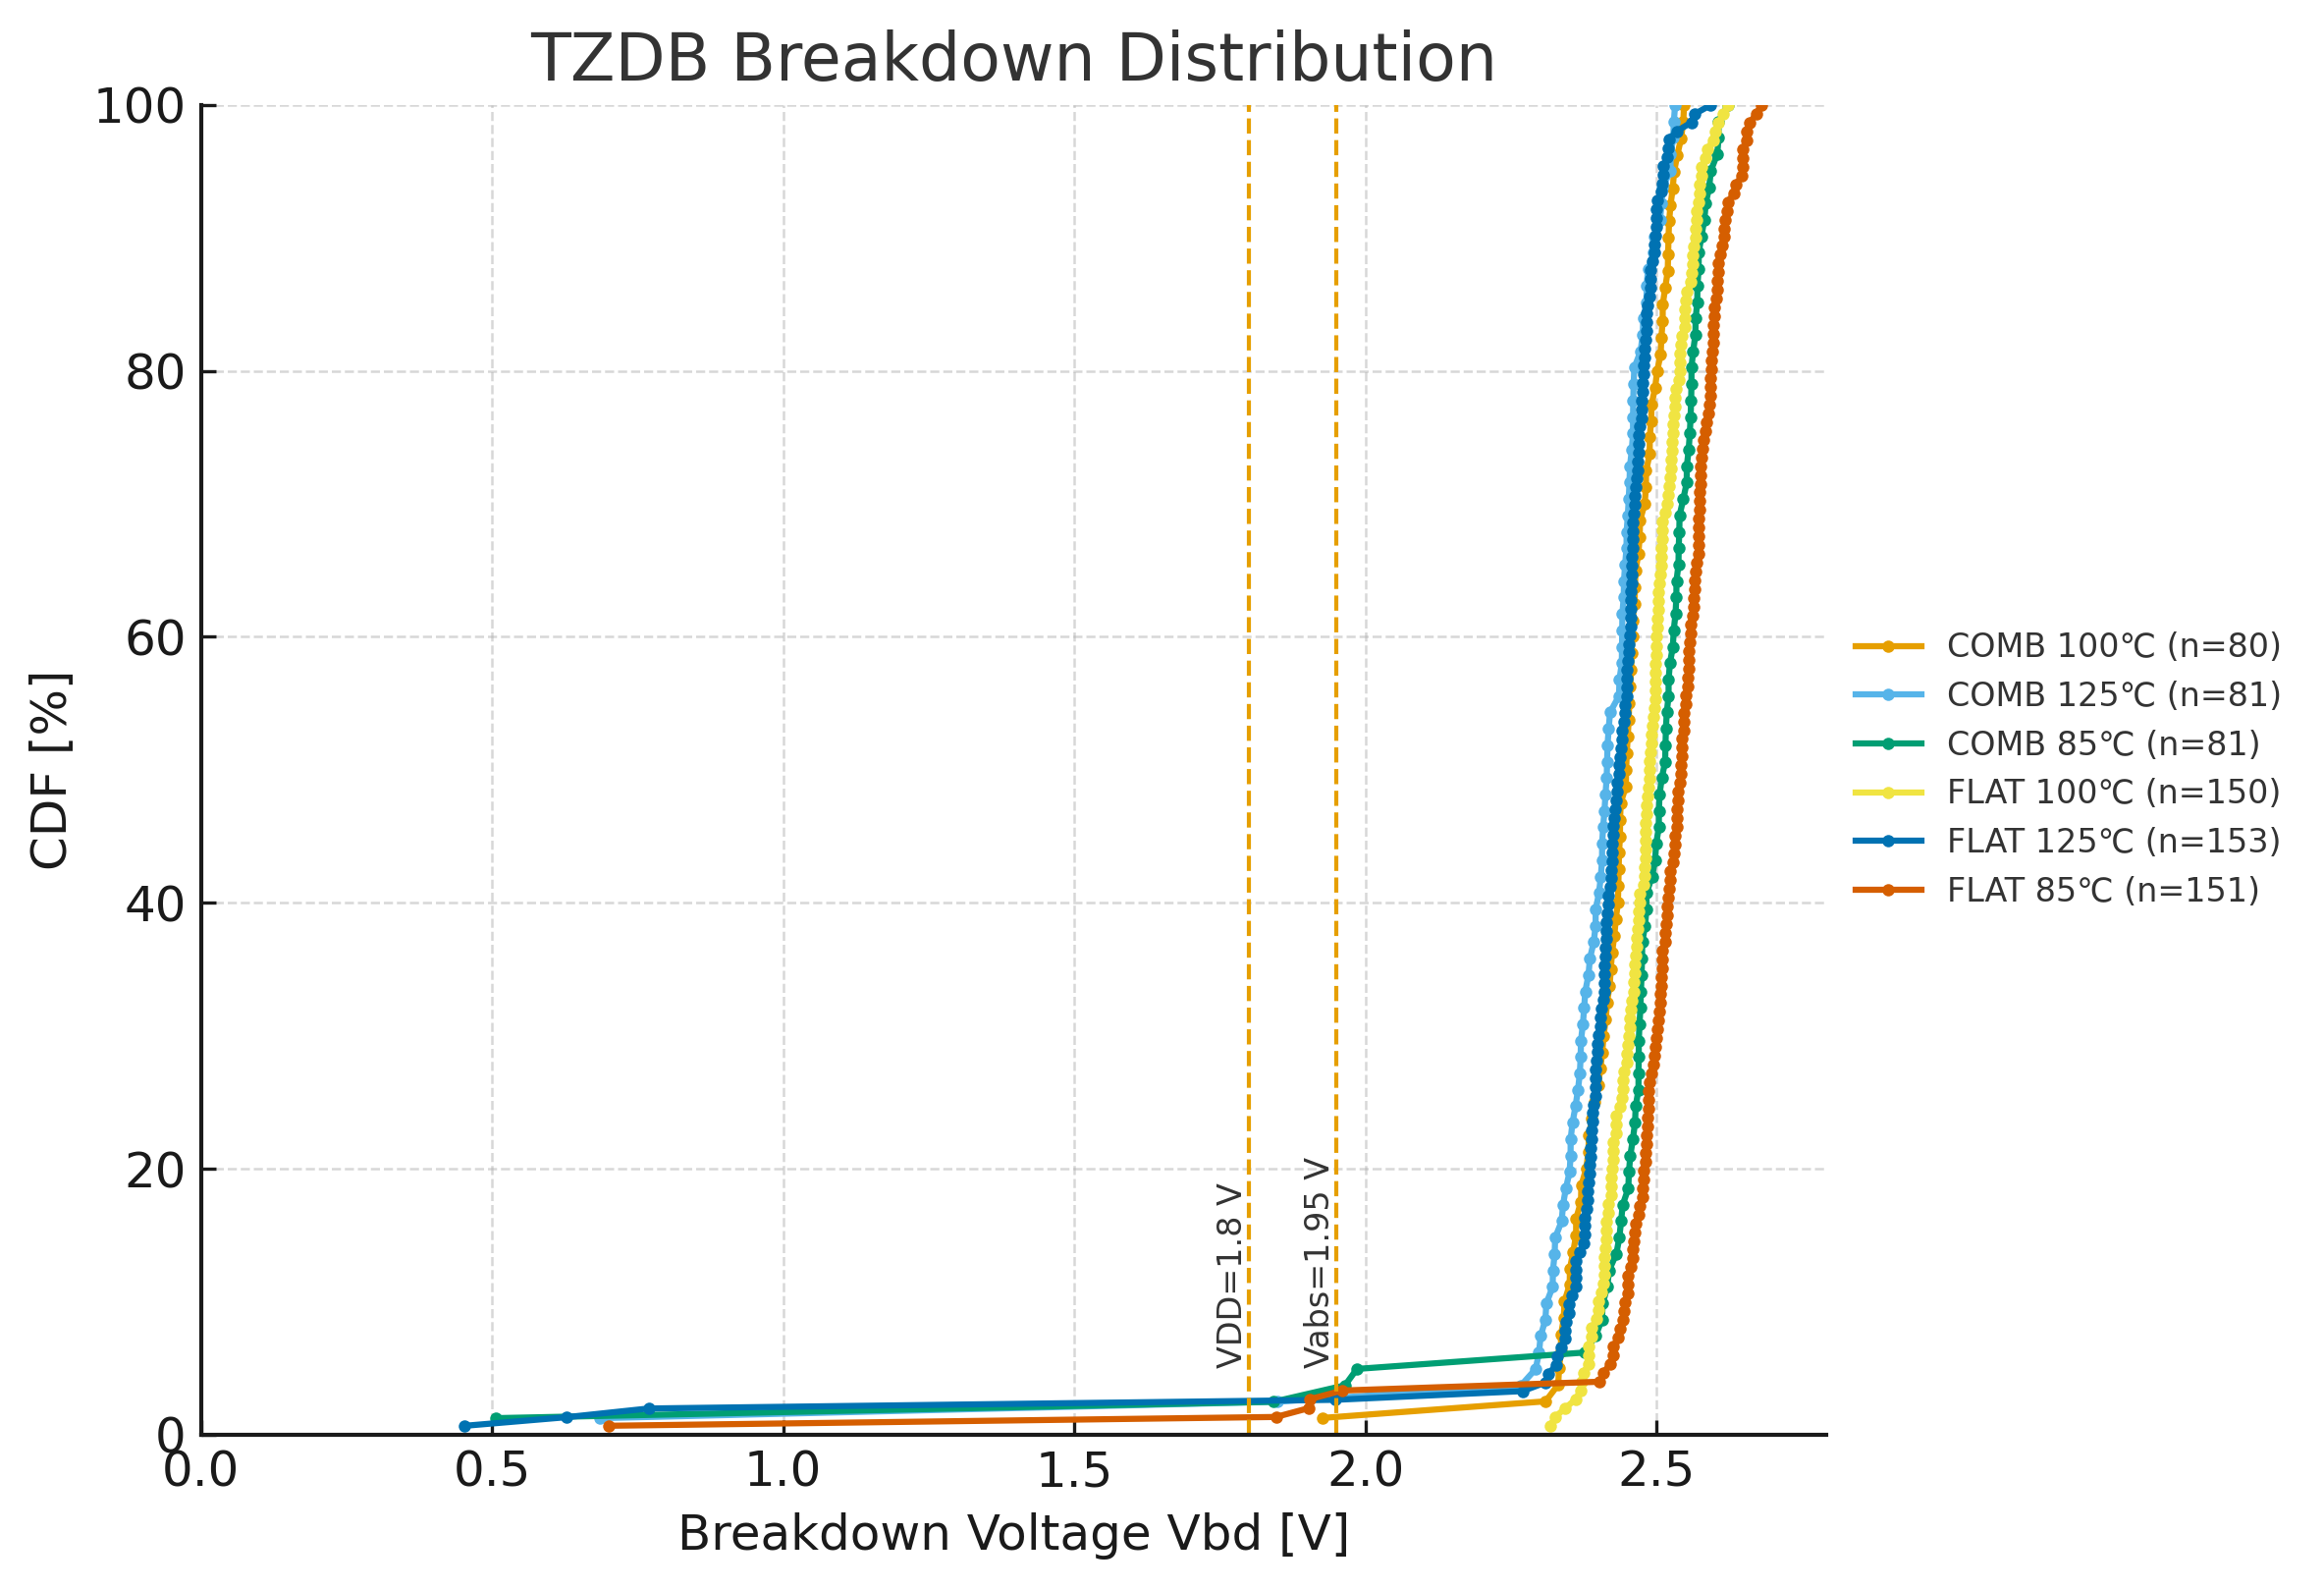
\includegraphics[width=\linewidth]{figures/fig3_tzdb.png}
  \caption{TZDB distributions of FeCAPs.}
  \label{fig:tzdb}
\end{figure}

\subsection{TDDB (Weibull/Arrhenius)}
Weibull analysis yields \(\beta \approx 1.3\) across stress conditions.  
The CDF and Weibull plots are shown in Fig.~\ref{fig:tddb_cdf} and Fig.~\ref{fig:tddb_weibull}.  
From scale parameters \(\eta\), Arrhenius fitting gives activation energies:
\(E_a\approx\SI{0.78}{eV}\) at 2.3~V, \(\SI{0.84}{eV}\) at 2.5~V, and \(\SI{0.88}{eV}\) at 2.7~V—consistent with oxygen-vacancy diffusion.

\begin{figure}[t]
  \centering
  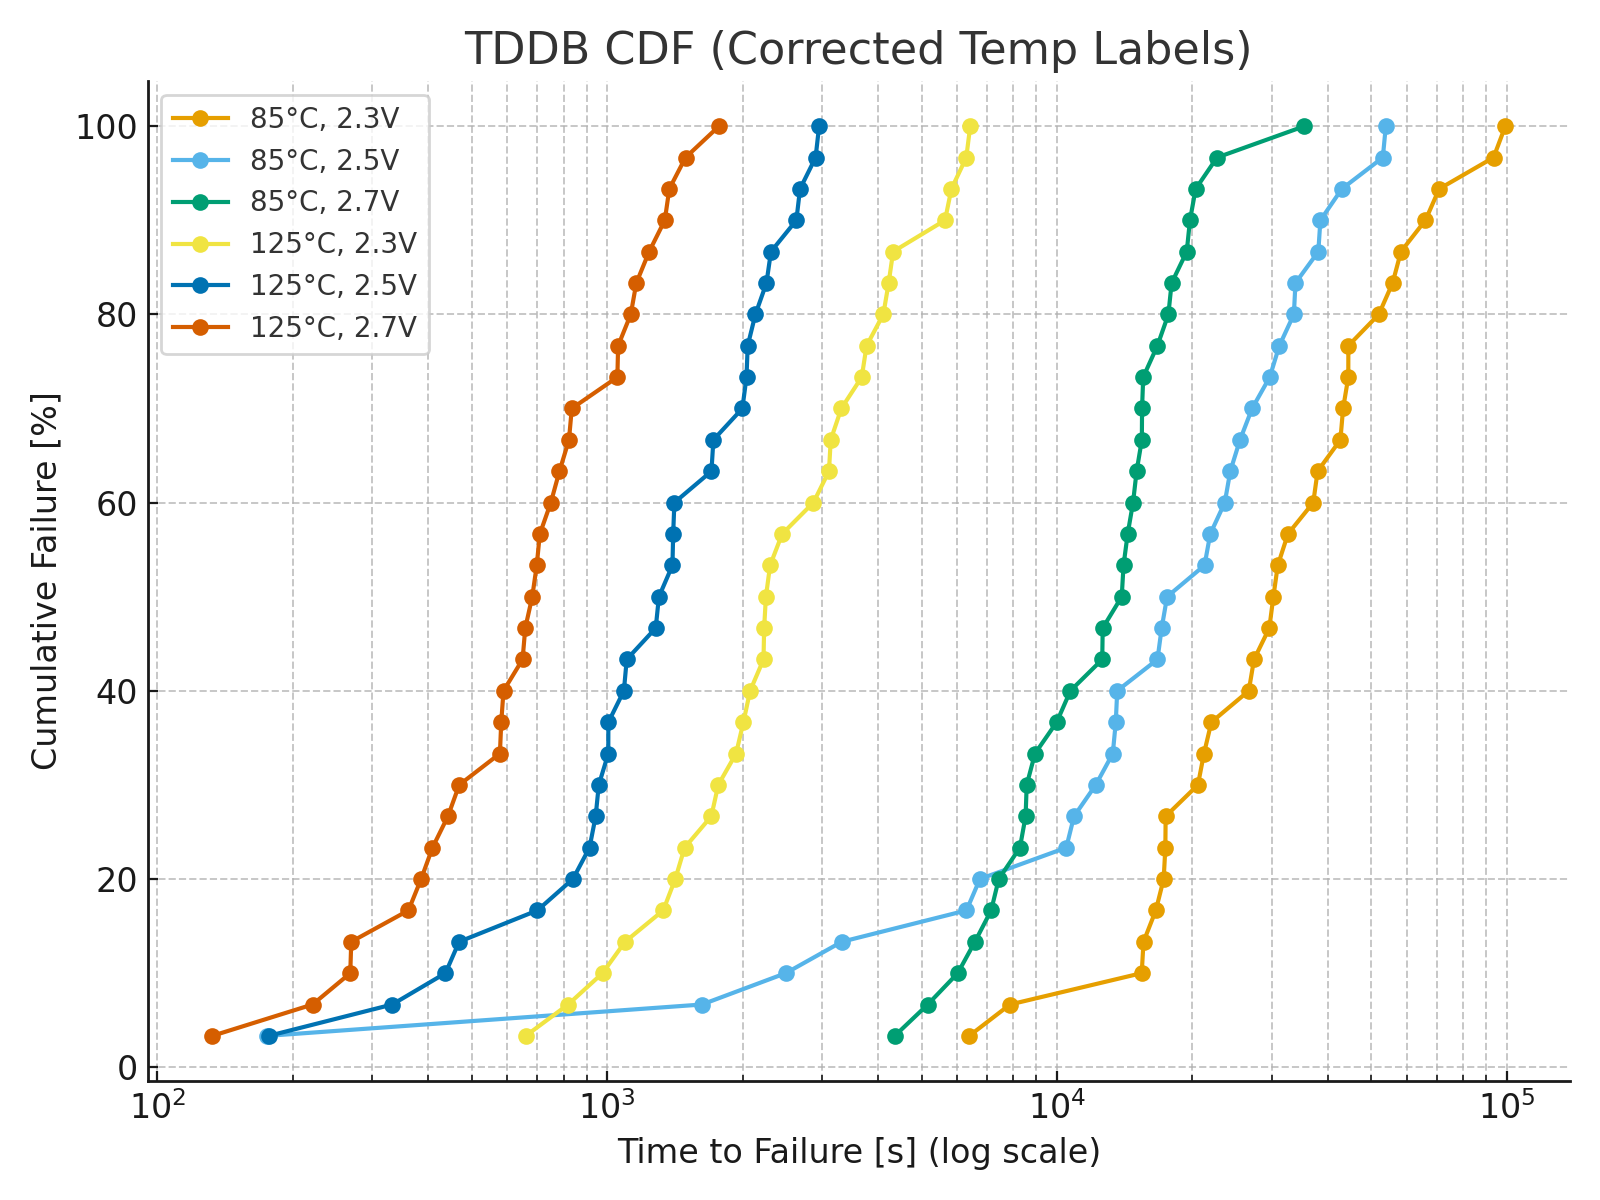
\includegraphics[width=\linewidth]{figures/fig4_tddb_cdf.png}
  \caption{TDDB CDF under all stress conditions.}
  \label{fig:tddb_cdf}
\end{figure}

\begin{figure}[t]
  \centering
  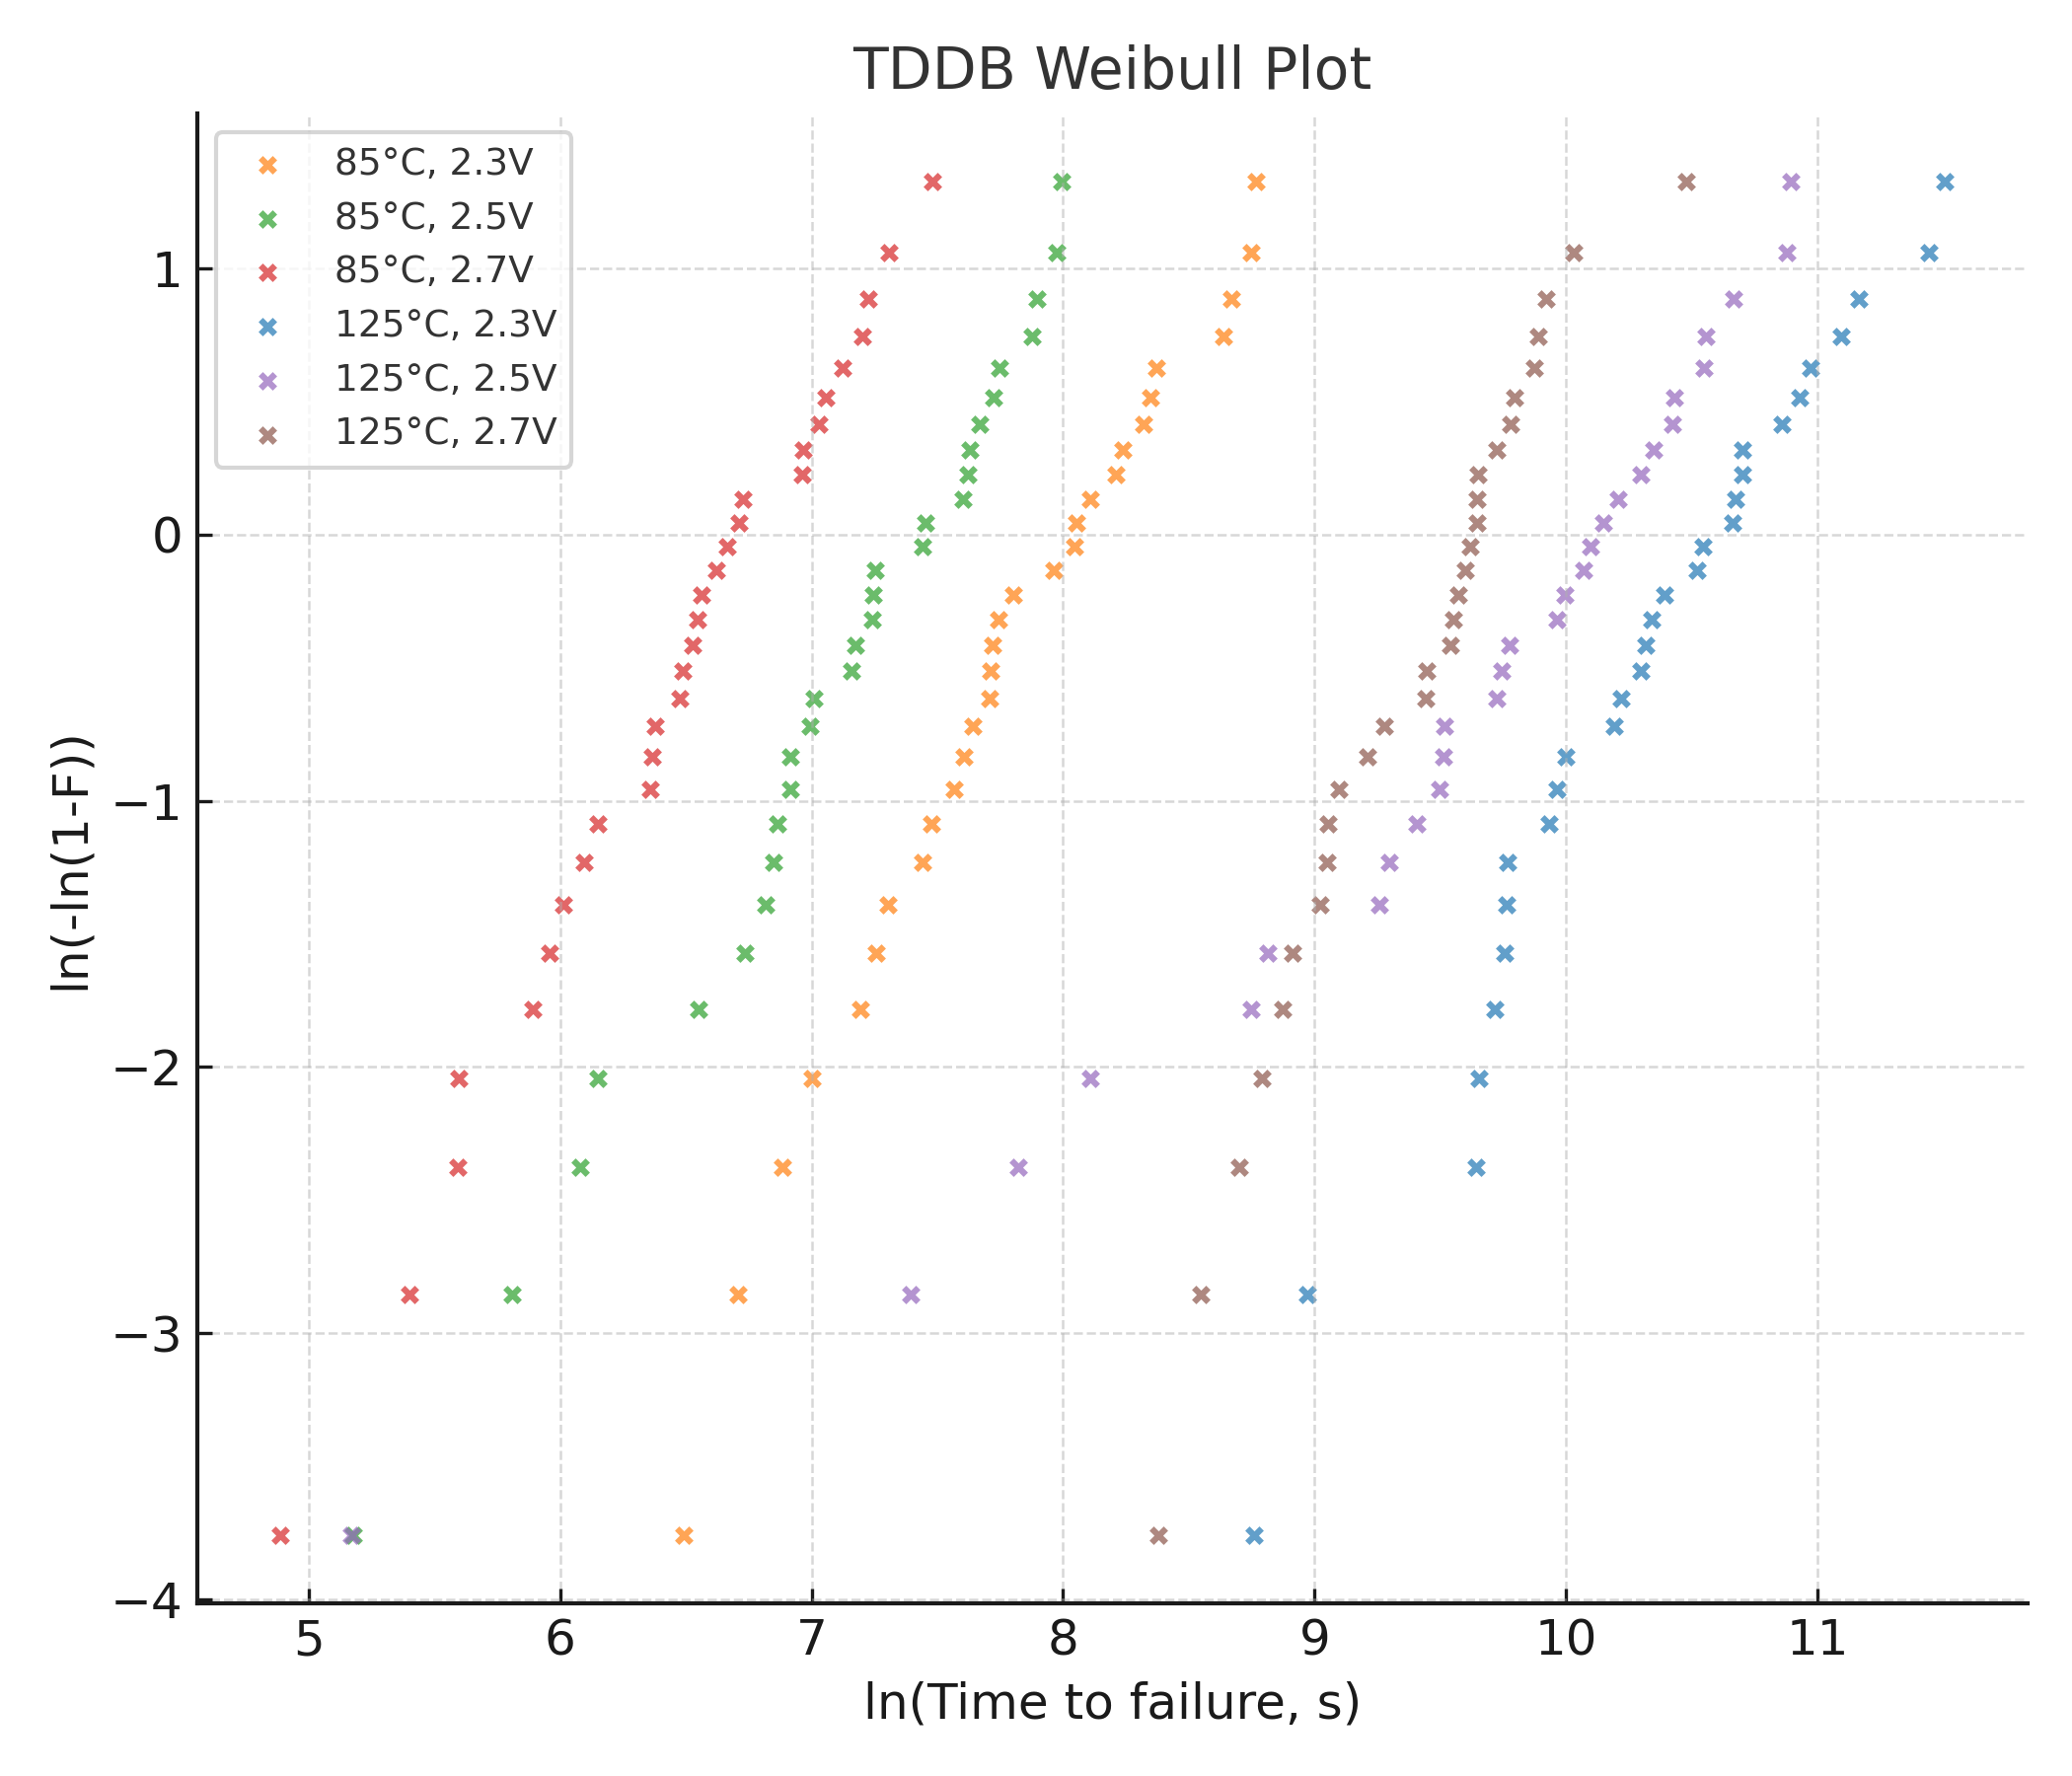
\includegraphics[width=\linewidth]{figures/fig4_tddb_weibull.png}
  \caption{TDDB Weibull plots with fitted lines (\(\beta,\eta\)).}
  \label{fig:tddb_weibull}
\end{figure}

\subsection{Endurance}
Up to \(10^{5}\) cycles were verified; the threshold window \(\Delta V_{\mathrm{th}}\) shrinks by roughly 20–30\%.  
A simple fit \(\Delta V_{\mathrm{th}}(N)=1.12-0.05\log_{10}N\) matches the trend (Fig.~\ref{fig:endurance}).

\begin{figure}[t]
  \centering
  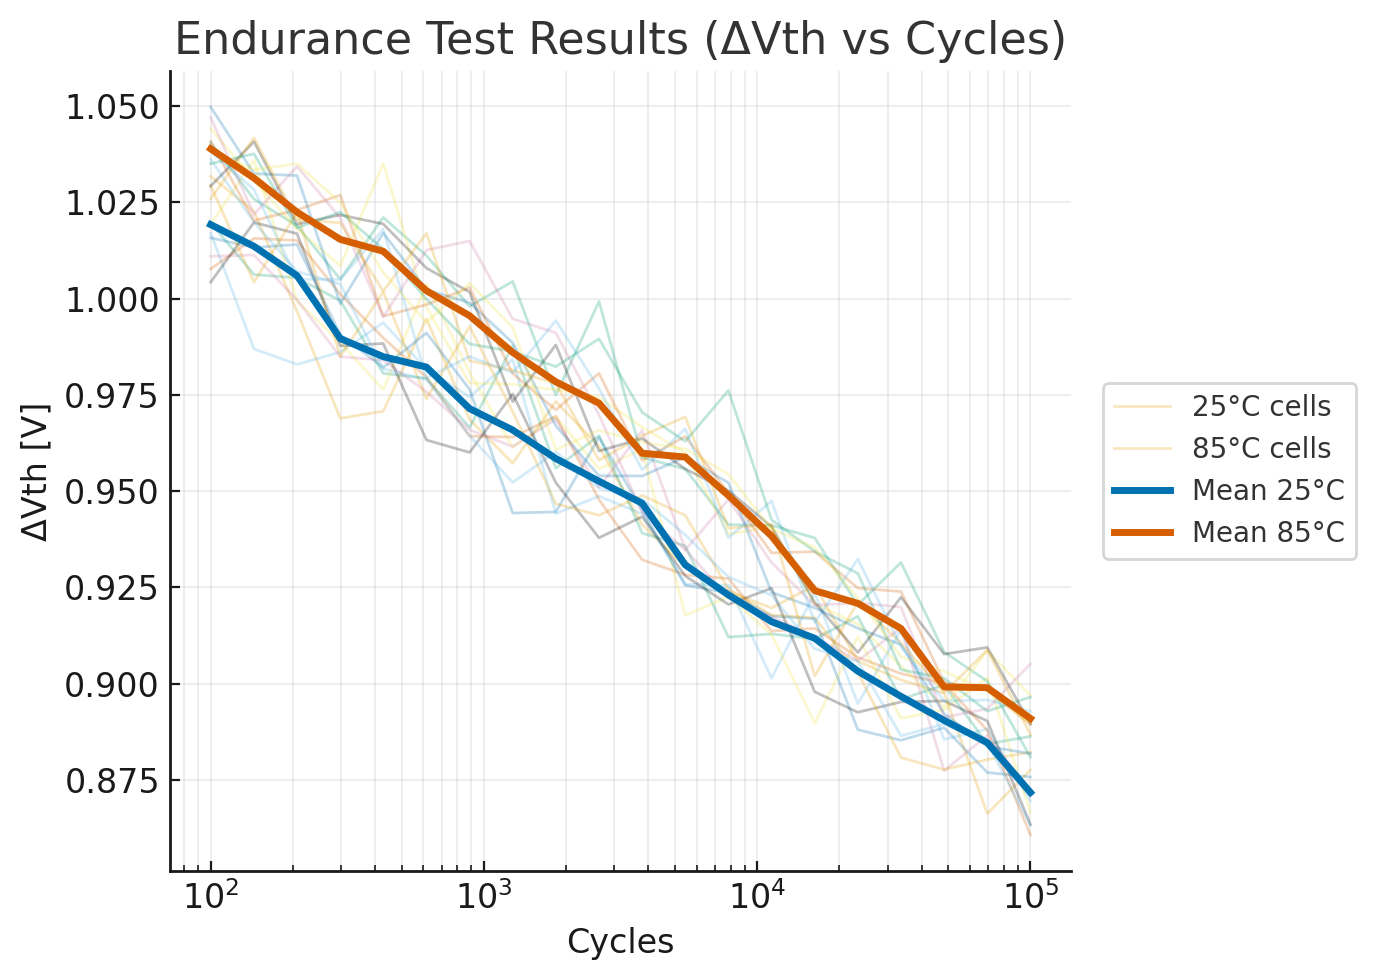
\includegraphics[width=\linewidth]{figures/fig5_endurance.png}
  \caption{Endurance characteristics (\(\Delta V_{\mathrm{th}}\) vs. cycles).}
  \label{fig:endurance}
\end{figure}

\subsection{Retention (Automotive View)}
Arrhenius extrapolation with \(E_a\approx\SI{1.1}{eV}\) predicts:
\(>\!10^{2}\) years at \SI{25}{\celsius}, \(>\!10\) years at \SI{85}{\celsius} (meets Grade-2), but only \(\sim\)months at \SI{150}{\celsius}; Grade-1/0 long-term targets are not yet met (Fig.~\ref{fig:retention}).

\begin{figure}[t]
  \centering
  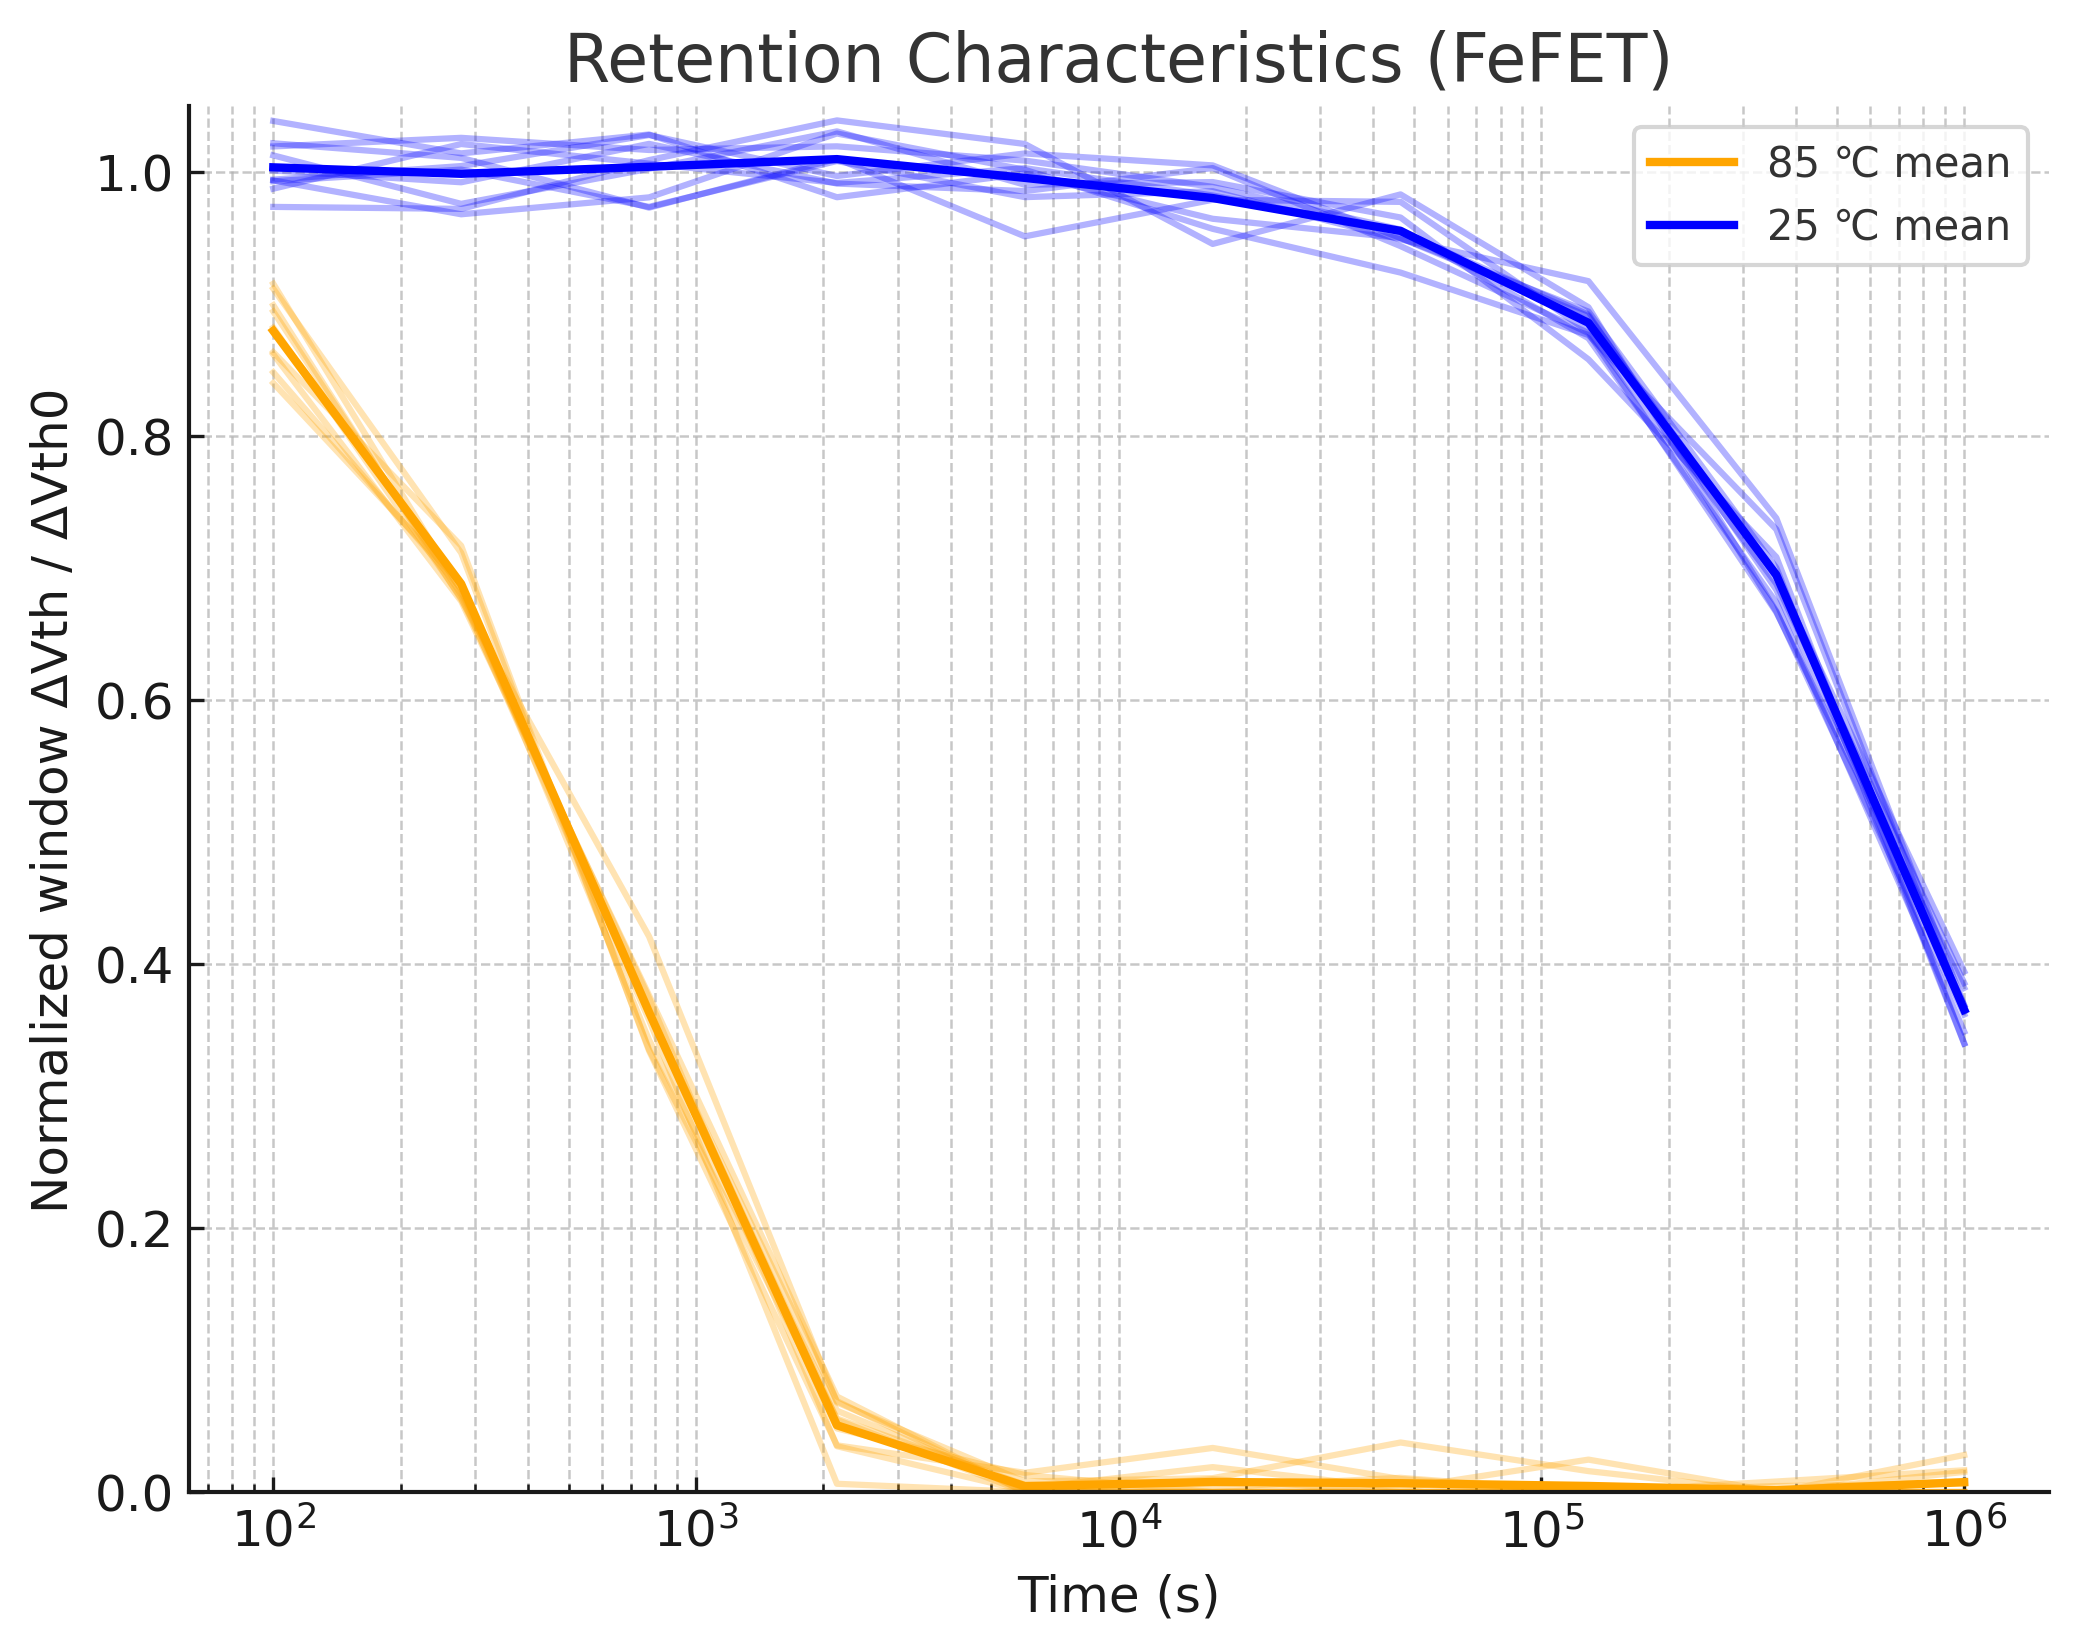
\includegraphics[width=\linewidth]{figures/fig6_retention.png}
  \caption{Retention characteristics and Arrhenius extrapolation.}
  \label{fig:retention}
\end{figure}

\section{Discussion}
The HZO/Al\(_2\)O\(_3\)/TiN stack provides sufficient reliability for industrial/consumer embedded NVM.  
For high-temperature automotive, improvements are required: (i) IL thickness optimization and HZO crystallinity control, (ii) refresh/rewrite operation, and (iii) ECC and redundancy.

\section{Conclusion}
We realized an FeFET module on \SI{0.18}{\micro m} CMOS with only \textbf{one extra mask} and \textbf{one ALD tool}. 
Devices exhibit \(>10^{5}\) cycles and \(>\!10\) years retention at \SI{85}{\celsius}. 
The method extends mature-node lifetime and enables cost-effective embedded NVM for automotive/industrial/IoT, while high-temperature retention remains the key item for Grade-1/0.

\section*{Acknowledgment}
The author thanks collaborators for helpful discussions.

\bibliographystyle{IEEEtran}
\begin{thebibliography}{99}
\bibitem{Boscke2011} T.~Böscke \emph{et al.}, \emph{Appl. Phys. Lett.}, vol.~99, p.~102903, 2011.
\bibitem{Mueller2012} J.~Müller \emph{et al.}, \emph{Appl. Phys. Lett.}, vol.~99, p.~112901, 2012.
\bibitem{Mikolajick2019} T.~Mikolajick \emph{et al.}, \emph{J. Appl. Phys.}, vol.~125, p.~204103, 2019.
\bibitem{Mueller2015} J.~Müller \emph{et al.}, \emph{IEEE Trans. Electron Devices}, vol.~62, no.~12, pp.~4158--4166, 2015.
\bibitem{Park2020} J.~Park \emph{et al.}, \emph{IEEE Electron Device Lett.}, vol.~41, no.~5, pp.~711--714, 2020.
\bibitem{Nakamura2003} H.~Nakamura \emph{et al.}, \emph{IEEE Trans. Device Mater. Rel.}, vol.~3, no.~4, pp.~132--136, 2003.
\bibitem{Yamazaki2018} K.~Yamazaki \emph{et al.}, \emph{Jpn. J. Appl. Phys.}, vol.~57, 04FB07, 2018.
\end{thebibliography}
\end{document}
